\RequirePackage{fix-cm}
\documentclass[11pt,a4paper,twoside]{vutinfth}

% useful packages
\usepackage{graphicx,
            textpos}
\usepackage{float}
\usepackage{helvet}
\usepackage{lipsum}
\usepackage{amsmath}
\usepackage{fancyhdr}
\usepackage{multicol}
\usepackage{setspace}
\usepackage[super, numbers]{natbib}
\usepackage{emptypage}
\usepackage[linktocpage=true]{hyperref}
\usepackage[toc,acronym,nonumberlist]{glossaries}
\usepackage{tocloft}
\usepackage{wrapfig}
\makeglossaries


% Import packages for drawing diagram
%More defined colors
\usepackage[dvipsnames]{xcolor}
% Required package
\usepackage{tikz}
\usetikzlibrary{positioning}

% Load packages to allow in- and output of non-ASCII characters.
\usepackage{lmodern}        % Use an extension of the original Computer Modern font to minimize the use of bitmapped letters.
\usepackage[T1]{fontenc}    % Determines font encoding of the output. Font packages have to be included before this line.
\usepackage[utf8]{inputenc} % Determines encoding of the input. All input files have to use UTF8 encoding.

% Extended LaTeX functionality is enables by including packages with \usepackage{...}.
\usepackage{amsmath}    % Extended typesetting of mathematical expression.
\usepackage{amssymb}    % Provides a multitude of mathematical symbols.
\usepackage{mathtools}  % Further extensions of mathematical typesetting.
\usepackage{microtype}  % Small-scale typographic enhancements.
\usepackage[inline]{enumitem} % User control over the layout of lists (itemize, enumerate, description).
\usepackage{multirow}   % Allows table elements to span several rows.
\usepackage{booktabs}   % Improves the typesettings of tables.
\usepackage{subcaption} % Allows the use of subfigures and enables their referencing.
\usepackage[ruled, lined, linesnumbered, commentsnumbered, longend]{algorithm2e} %
%Enables the writing of pseudo code.
%\usepackage[usenames,dvipsnames,table]{xcolor} % Allows the definition and use o colors.
%This package has to be included before tikz.
\usepackage{nag}       % Issues warnings when best practices in writing LaTeX documents are violated.
\usepackage{todonotes} % Provides tooltip-like todo notes.
\usepackage{hyperref}  % Enables cross linking in the electronic document version. This package has to be included second to last.
\usepackage[acronym,toc]{glossaries} % Enables the generation of glossaries and lists fo acronyms. This package has to be included last.

% Define convenience functions to use the author name and the thesis title in the PDF document properties.
\newcommand{\authorname}{Jan Stevens} % The author name without titles.
\newcommand{\thesistitle}{Coarse grained simulations of the DNA nanopistion} % The title

% Set PDF document properties
\hypersetup{
    pdfpagelayout   = TwoPageRight,           % How the document is shown in PDF viewers (optional).
    pdfauthor       = {\authorname},          % The author's name in the document
    pdftitle        = {\thesistitle},         % The document's title in the document
    pdfsubject      = {Master Thesis: Jan Stevens},              % The document's subject
    pdfkeywords     = {Thesis, Physics, DNA, Simulations}, % The document's keywords in
    colorlinks      = true,
    allcolors       = blue,
    linkbordercolor = {white}
}

\setpnumwidth{2.5em}        % Avoid overfull hboxes in the table of contents (see memoir

\setsecnumdepth{subsection} % Enumerate subsections.

\nonzeroparskip             % Create space between paragraphs (optional).
\setlength{\parindent}{0pt} % Remove paragraph identation (optional).

\makeindex      % Use an optional index.
\makeglossaries % Use an optional glossary.
\glstocfalse   % Remove the glossaries from the table of contents.


% settings for table of contents and section numbering
\setcounter{secnumdepth}{1} % numbering to which sublevel?
\setcounter{tocdepth}{1} % How many levels does the table of contents have?

\newcommand*\cleartoleftpage{%
  \clearpage
  \ifodd\value{page}\hbox{}\newpage\fi
}

% page settings
%\topmargin -10mm
%\textwidth 160truemm
%\textheight 240truemm
%\oddsidemargin 0mm
%\evensidemargin 0mm


% define the KUL colors
\definecolor{green}{RGB}{172,196,0}
\definecolor{bluetitle}{RGB}{29,141,176}
\definecolor{blueaff}{RGB}{0,0,128}
\definecolor{blueline}{RGB}{82,189,236}

% define units for the text blocks
\setlength{\TPHorizModule}{1mm}
\setlength{\TPVertModule}{1mm}

% Define your symbols and acronyms in here
% Used to give a list of symbols in Glossary on page vii
\newglossaryentry{pi}
{
  name={\ensuremath{\pi}},
  description={ratio of circumference of circle to its
               diameter},
  sort=pi
}

\newglossaryentry{alpha}
{
  name={\ensuremath{\alpha}},
  description={a random greek letter},
  sort=alpha
}

% Used to give a list of Acronyms in Acronyms on page ix
\newacronym{LSS}{LSS}{landslide susceptibility}


% Remove rule and put quote on the left of page
\renewcommand{\epigraphflush}{center}
%\renewcommand{\epigraphflush}{flushleft}

\epigraphfontsize{\small\itshape}
\setlength\epigraphwidth{9cm}
\setlength\epigraphrule{1pt}

\newenvironment{smallfont}{\fontfamily{lmodern}\small\selectfont}{\par}

% Start of the actual document
\begin{document}

\selectlanguage{english}

\newcommand\mycommfont[1]{\small\ttfamily\textcolor{blue}{#1}}
\SetCommentSty{mycommfont}

% FRONT MATTER
\frontmatter
\rmfamily

\thispagestyle{empty}
\newcommand{\form}[1]{\scalebox{1.087}{\boldmath{#1}}}
\sffamily
%
\begin{textblock}{191}(-17,-20)
    \colorbox{green}{\hspace{123mm}\
    \hspace{20mm}\parbox[c][18truemm]{48mm}{\textcolor{white}{FACULTY OF SCIENCES}}}
\end{textblock}
%
\begin{textblock}{70}(-11,-27)
\textblockcolour{}
\includegraphics*[height=19.8truemm]{Figures/LogoKULeuven}
\end{textblock}
%
\begin{textblock}{160}(-6,26)
\textblockcolour{}
\vspace{-\parskip}
\flushleft
\fontsize{40}{38}\selectfont \textcolor{bluetitle}{Coarse-grained simulations of the DNA
nanopiston}\\[1.5mm]
%\fontsize{20}{22}\selectfont subtitle \form{$S=\pi r^2$\textsl{(optional)}}
\end{textblock}
%
%\begin{textblock}{160}(8,147)
%\textblockcolour{}
%\vspace{-\parskip}
%\flushright
%\fontsize{14}{16}\selectfont \textbf{Jan Stevens}
%\end{textblock}
%
\begin{textblock}{160}(8,161)
\textblockcolour{}
\vspace{-\parskip}
\flushright
\fontsize{14}{16}\selectfont \textbf{Jan Stevens}
\end{textblock}
%
\begin{textblock}{70}(-6,185)
\textblockcolour{}
\vspace{-\parskip}
\flushleft
Supervisor: Prof. E. Carlon\\[-2pt]
\textcolor{blueaff}{Affiliation \textsl{(optional)}}\\[5pt]
Tutor: \textsl{(optional)}\\[-2pt]
\textcolor{blueaff}{Affiliation \textsl{(optional)}}\\
\end{textblock}
%
\begin{textblock}{160}(8,185)
\textblockcolour{}
\vspace{-\parskip}
\flushright
Thesis presented in\\[4.5pt]
fulfillment of the requirements\\[4.5pt]
for the degree of Master of Science\\[4.5pt]
in Physics
\end{textblock}
%
\begin{textblock}{160}(8,224)
\textblockcolour{}
\vspace{-\parskip}
\flushright
Academic year 2020-2021
\end{textblock}
%
\begin{textblock}{191}(-17,237)
{\color{blueline}\rule{550pt}{5.5pt}}
\end{textblock}
%
%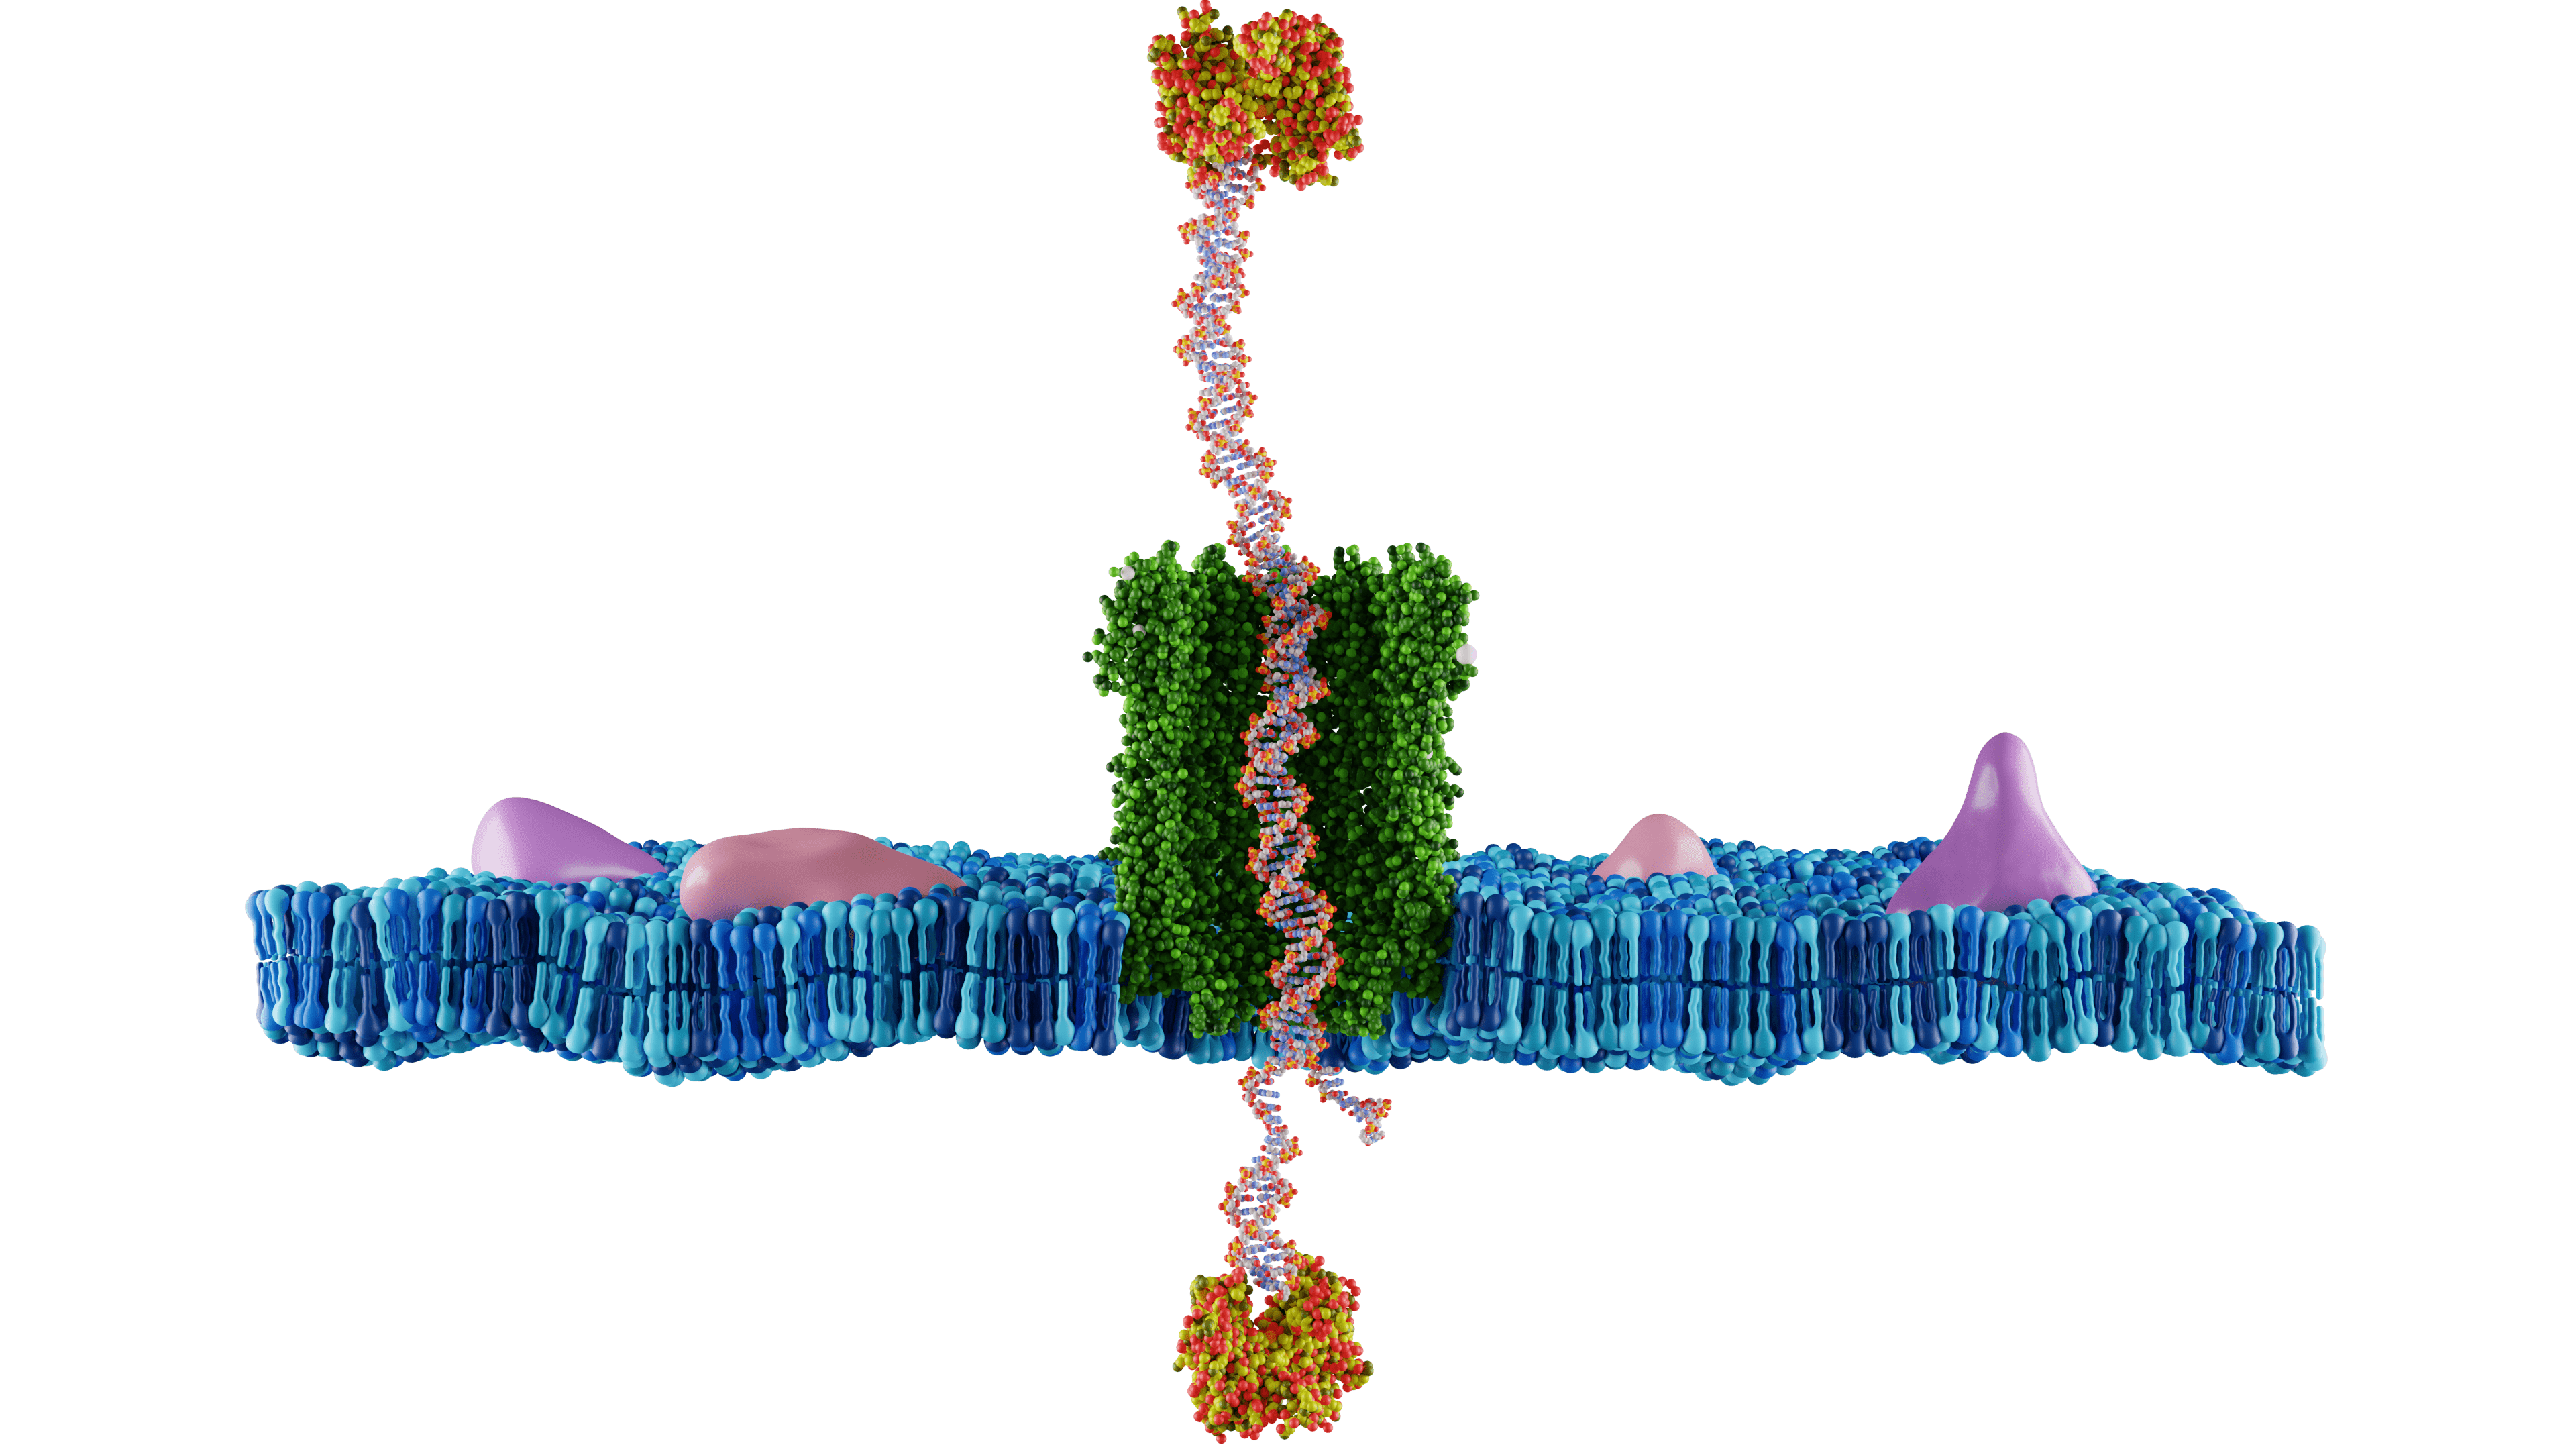
\includegraphics[height=9.5cm, width = 15.5cm]{Figures/CoverPhoto.png}
\vspace*{5.7cm}
\begin{center}
\begin{figure}[H]
\centering
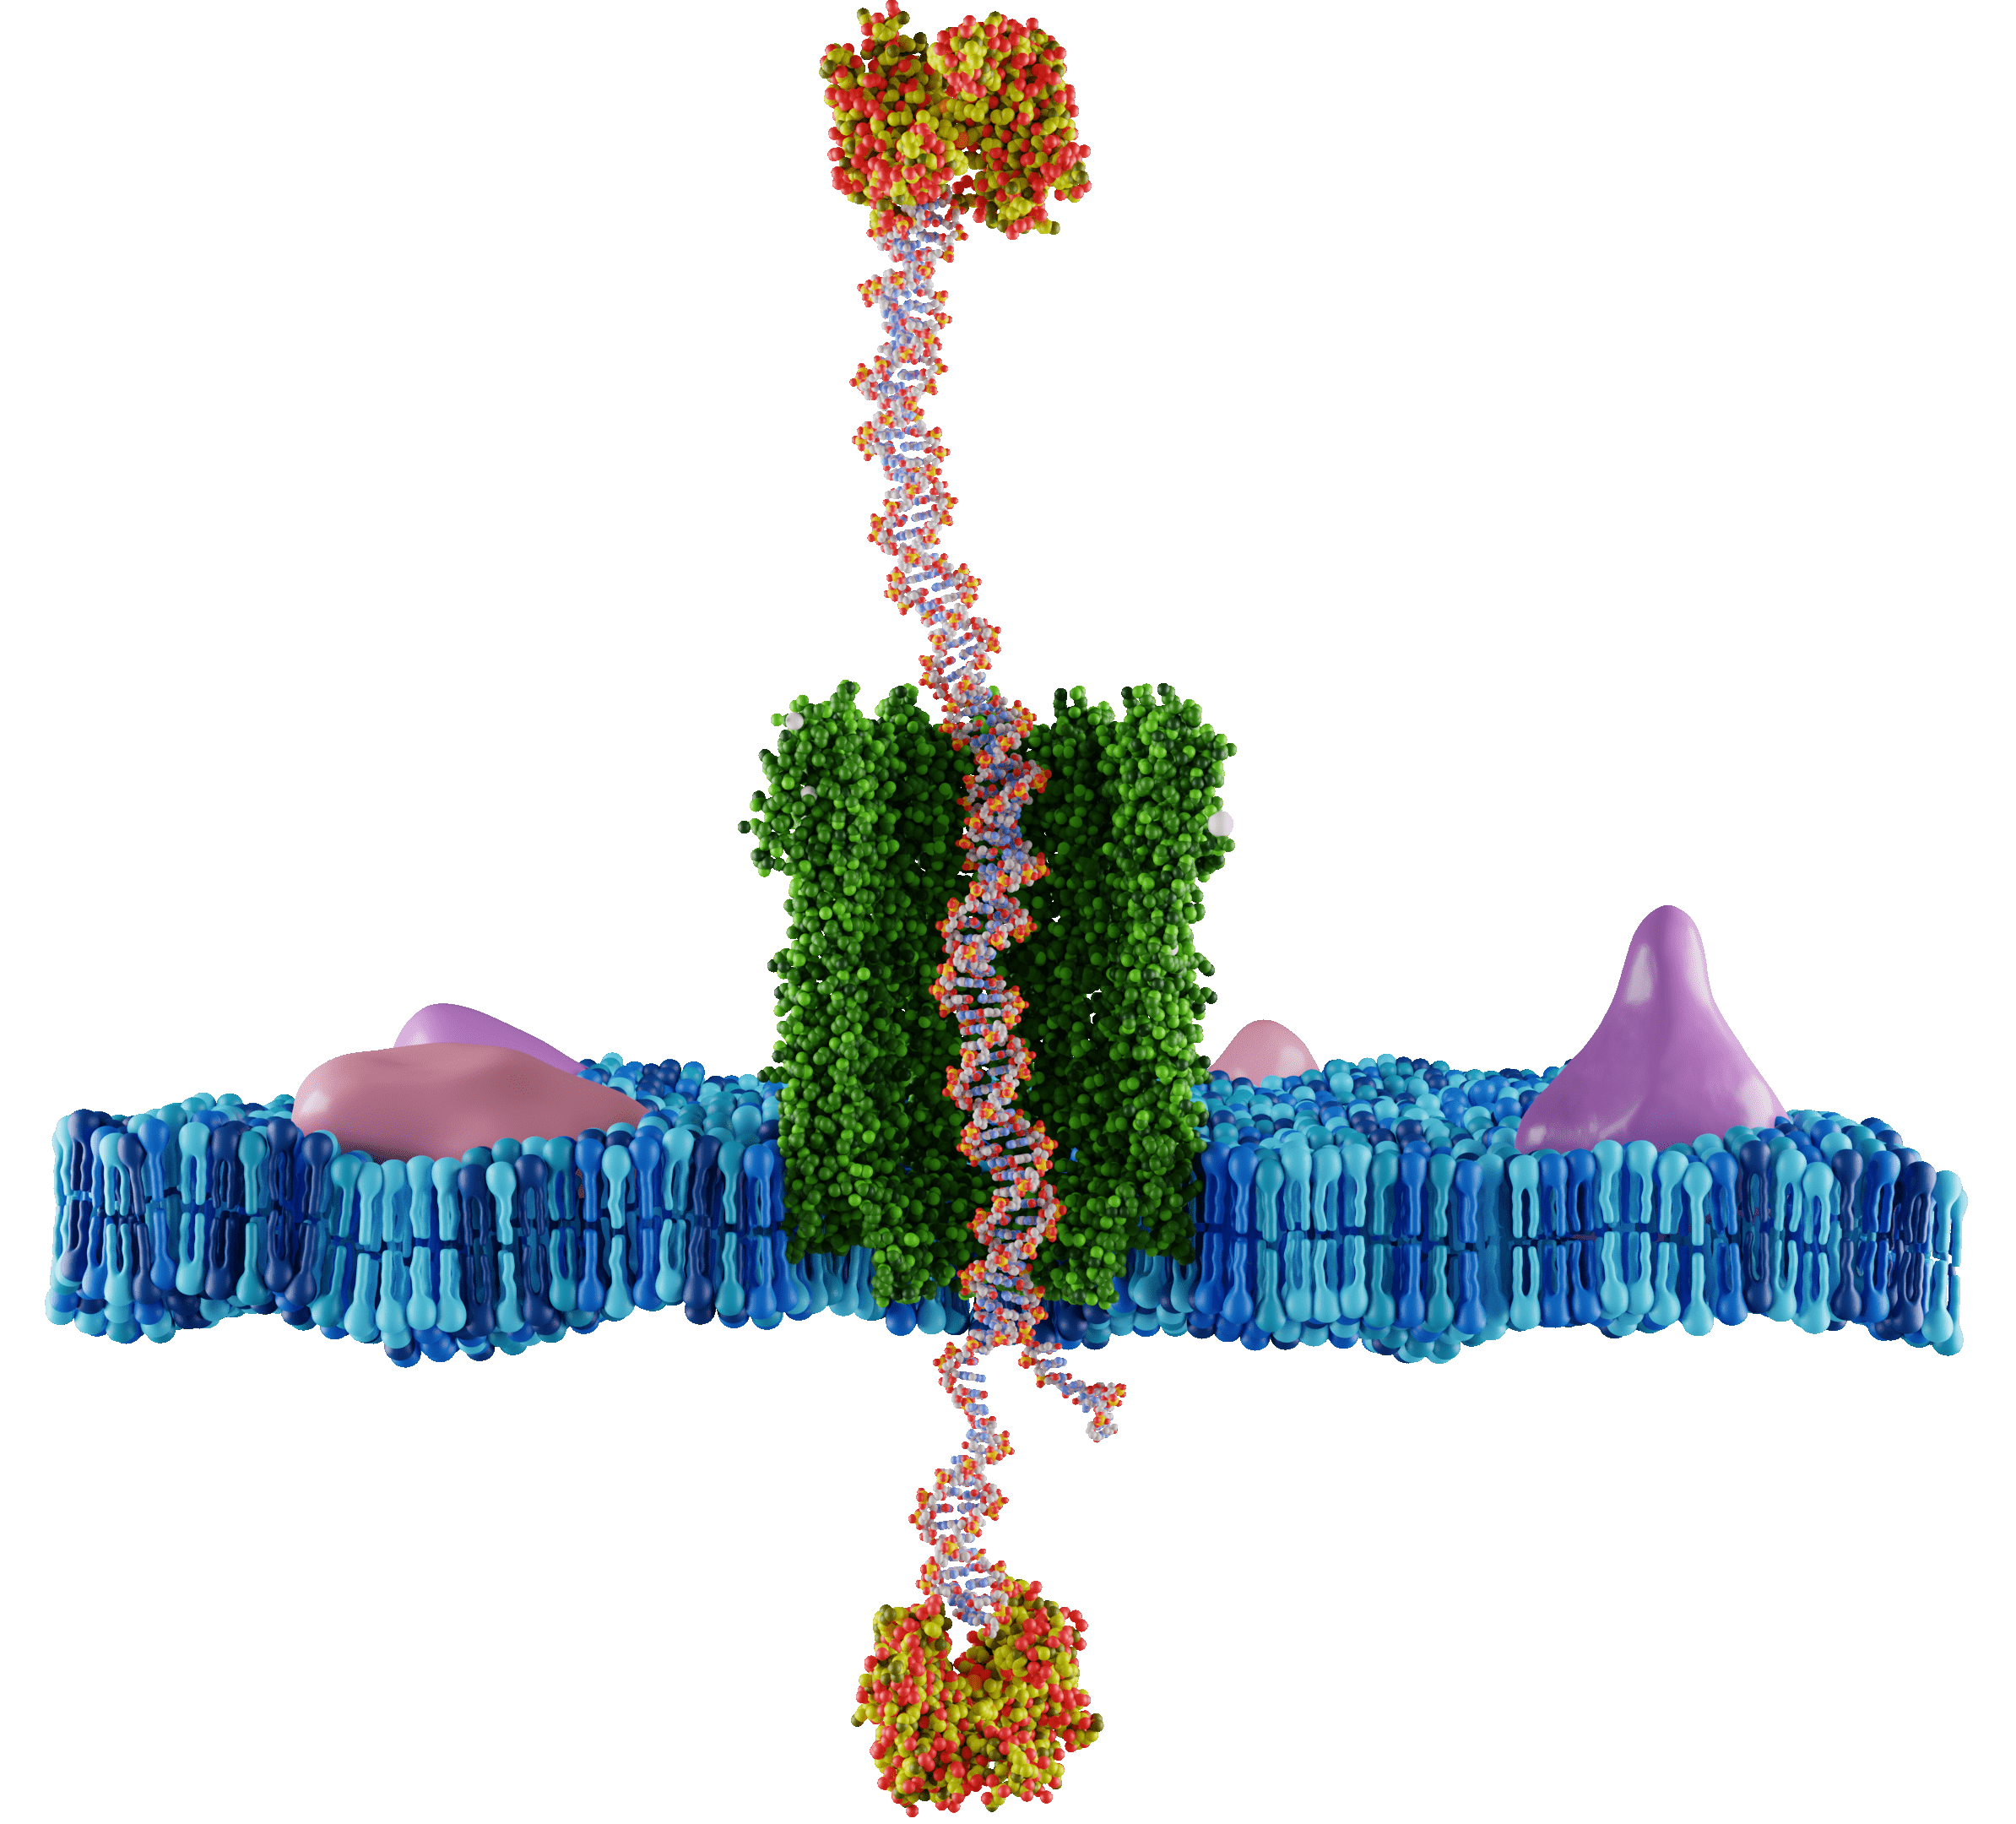
\includegraphics[scale=0.166]{Figures/CoverPhoto2.png}
\end{figure}
\end{center}
%
\vfill
 \cleardoublepage
\thispagestyle{empty}
\setlength{\parindent}{0cm}
\vspace*{\fill}

\begin{smallfont}
\copyright\ Copyright by KU Leuven \par
Without written permission of the promoters and the authors it is forbidden to reproduce or adapt in any form or by any means any part of this publication. Requests for obtaining the right to reproduce or utilize parts of this publication should be addressed to KU Leuven, Faculteit Wetenschappen, Geel Huis, Kasteelpark Arenberg 11 bus 2100, 3001 Leuven (Heverlee), Telephone +32 16 32 14 01.
A written permission of the promoter is also required to use the methods, products, schematics and programs described in this work for industrial or commercial use, and for submitting this publication in scientific contests.
\end{smallfont}

\setlength{\parindent}{0.5cm}
 \cleardoublepage
\setcounter{page}{0}
\pagenumbering{roman}

\addcontentsline{toc}{chapter}{Abstract}
\chapter*{Abstract}

Autonomous molecular machines are ubiquitous in the machinery of life, collectively
driving the molecular processes in our cells. Inspired by these biological machines,
scientists
develop synthetic devices performing specialised operations at the nanoscale. In this
thesis we study a specific molecular machine designed by Bayoumi et al.\cite{Bayoumi21},
which is composed of a DNA-neutravidin piston trapped inside a ClyA nanopore.

Using the free energy of DNA hybridisation this molecular machine is able to perform
autonomous and active transport of DNA cargo both following or opposing an
external bias force. During each operating cycle of the nanopiston a DNA cargo
is transported from the cis- to the trans-side of the membrane, in which the piston is
embedded.

Due to the length scale associated with molecular machines performing in depth
experimental studies has been proven to be challenging. During this thesis we aim
to shed light on the operating principles of the nanopiston by using molecular dynamics
simulations. Motivated by the computational cost of classical all-atom simulations a
coarse-grained model of the DNA nanopiston is designed.

Entropic interactions between the DNA piston and the nanopore are thought to
play an important role in facilitating the DNA transport. Studying these effects reveal
two distinct origins of entropic forces. Large double stranded DNA is kept predominantly
outside of the pore's constriction, by the entropic penalty of confinement.  Whereas, the
flexible single stranded DNA also
endouvours to maximize its available configurational space by opposing confinement.

Consecutively the  conformational fluctuations of
the nanopiston are studied.  These simulations clearly show the importance of the
entropic interactions promoting the operation cycle.  The entropic
penalty of confining the flexible single stranded DNA components of the piston in the
nanopore enable the continuation of the hybridisation reactions.

In an attempt to study a full piston cycle, the hybridisation reactions driving the
operation are simulated using our coarse-grained
model. Due to the inherent difficulty of simulating these reactions an advanced
sampling method called forward flux sampling is needed.
While performing these simulations the main limitation of our coarse-grained model is
encountered. The compliance of the biological nanopore is found to be essential in
facilitating the hybridisation pathways, but is not yet incorporated in our current
model.

\cleardoublepage
\cleardoublepage
\addcontentsline{toc}{chapter}{Samenvatting}
\chapter*{Samenvatting}
Summary in dutch.

\cleardoublepage
\addcontentsline{toc}{chapter}{Summary}
\chapter*{Summary}
Summary in english.
 \cleardoublepage
\printglossaries \cleardoublepage
%\addcontentsline{toc}{chapter}{List of Figures}
\listoffigures \cleardoublepage
%\addcontentsline{toc}{chapter}{List of Tables}
\listoftables \cleardoublepage
%\addcontentsline{toc}{chapter}{Contents}
\linespread{0.9}
{\small \tableofcontents}
\cleardoublepage
\linespread{1}

% MAIN MATTER
\mainmatter
\setcounter{page}{0}
\pagenumbering{arabic}

\chapter{Introduction}
\vspace{-1cm}
\epigraphfontsize{\small\itshape}
\epigraph{“...if we were to name the most powerful assumption of all, which leads one on
and on in an attempt to understand life, it is that all things are made of atoms, and
that everything that living things do can be understood in terms of the jigglings and
wigglings of atoms.”}
{--- \textup{Richard P. Feynman}, The Feynman Lectures on Physics\cite{feynmanLectures}}

\section{Deoxyribonucleic Acid}

\section{Polymer Physics}

\newpage

\section{Computer Simulations}

The theory of classical mechanics is often regarded as the first major breakthrough in
the field of physics. For every aspiring physicist this is still the starting point of
their studies. Unfortunately getting to know these relatively simple laws of nature,
leads to the inescapable realisation that these theories are expressed in mathematical
formalism that are only analytically solvable in few idealised scenarios. Applying these
formulas to a problem consisting of just more then two particles already leads
practically unsolvable equations.\\

Although it is often times not possible to find an exact solution to equations
related to complex physical systems, finding reasonable approximations to their solution
is. One popular method to analyse the dynamics of complex systems is the use of
simulations.\\

\begin{wrapfigure}{r}{0.5\textwidth}
  \begin{center}
    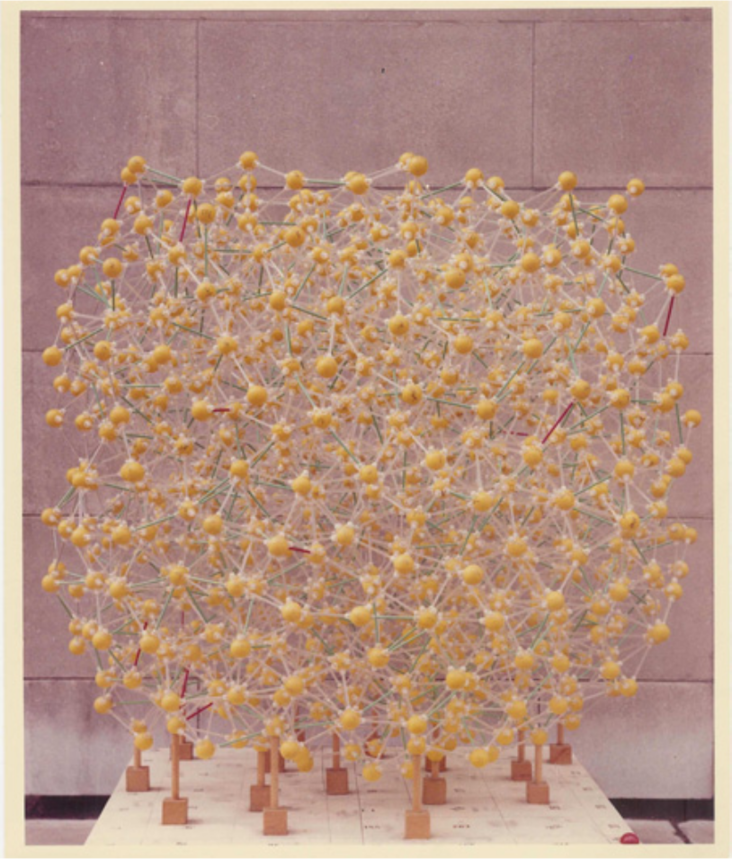
\includegraphics[width=0.38\textwidth]{Figures/WaterModel.png}
  \end{center}
  \caption{Example of an expanded model of a simple liquid (J L Finney, Ph.D thesis)}
\end{wrapfigure}

Simulations have a rich history within physics and engineering, starting even before the
invention of the computer. An example of one of these mechanical simulations is the
 Waterloopkundig Laboratorium or currently the waterloopbos, a scale model of important
Dutch waterways where the influence of waves on harbours and docks was studied. This
simulation played an important part in the design of the famous Delta Works.\\
Another example is the use of mechanical simulations to study the structure of water. In
the early 20th century physicist J.D. Bernal and his fellow researches build various ball
and stick models of water to analyse the possible 3D configurations of water molecules in
a liquid. Their research eventually explained the peculiar physical properties
of water from a atomistic perspective. However useful these mechanical simulations turned
out to be, the biggest drawback of the method was the extreme cost of labour to construct
them as pointed out by Bernal in his 1962 lecture,

\begin{quote}
\dots I took a number of rubber balls and stuck them together with rods of a
selection of different lengths ranging from 2.75 to 4 inch. I tried to do this in the
first place as casually as possible, working in my own office being interrupted every
five minutes or so and not remembering what I had done before the interruption.
However,\dots
\end{quote}

After the first computer simulations where performed in the Los Alamos labs, the
popularity of simulations rapidly increased. The remarkable explanatory power of
simulations combined with the relative easy construction of computer models lead to a
fast adoption of computer simulations in the scientific community. Within the context of
this thesis, computer simulations are used to study the mechanics of
the DNA Polymer. Due to the high number of atoms in a typical system, it is generally
not possible to find an analytical solution to their equations of motion. In this
context, simulations are often used to gain an insight into the complex dynamics of the
system and guide the developments of simple approximate theories. The simulations
act as a bridge between the microscopic constituents of the systems and the macroscopic
properties we want to understand.


\subsection{Molecular Dynamics Simulations}
Molecular Dynamics (MD) is a computer simulation technique, used to analyse
the dynamics of a classical many-body system. The central idea of this method is to
generate all the particle trajectories in a system of N particles by numerically
integrating the classical equations of motion,
\[
    m_i \boldsymbol{\ddot{r_i}} = \boldsymbol{f_i}, \quad \boldsymbol{f_i} = -
    \frac{\partial}{\partial \boldsymbol{r_i}} \mathcal{U}, \quad for\ i \in N.
\]
Solving these differential equations is then achieved by employing a discretized time
integration scheme.  Algorithm 1 shows the typical structure of a molecular dynamics
simulations. The discretization resolution is conventionally called the time step of the
simulations denoted by $\Delta t$. The integration scheme we use depends on the system we
want simulate. For Isolated systems an energy conserving integration scheme is needed, a
popular example is the velocity-Verlet algorithm is. If on the other hand a

- thermostats

- Integrations schemes

- Rare event sampling

\begin{algorithm}
    \SetKwFunction{isOddNumber}{isOddNumber}
    \SetKwInOut{KwIn}{Input}
    \SetKwInOut{KwOut}{Output}

    \KwIn{Configuration of the system at $t=0$}
    \KwOut{Configuration of the system at $t=t_{f}$}

    $newList = [\ ]$

    \tcc{For odd elements in the list, we add 1, and for even elements, we add 2.
    After the loop, all elements are even.}
    \For{$i \leftarrow 0$ \KwTo $n-1$}{
        \eIf{$\isOddNumber(a_i)$}{

            $newList.append(a_i + 1)$ \tcp*[f]{Some thought-provoking comment.}
         }{
            \tcp{Another comment}
            $newList.append(a_i + 2)$
         }
    }

    \KwRet{$newList$}
    \caption{The Velocity Verlet algorithm}
\end{algorithm}

% \begin{center}
% 	\begin{tikzpicture}[
% 	squarednode/.style={rectangle, draw=blue!60, fill=blue!5, very thick, minimum width=50mm,
% 	minimum height=5mm},]
% 	%Nodes
% 	\node[squarednode]      (step1)                        {1};
% 	\node[squarednode]      (step2)       [below= 3mm of step1] {2};
% 	\node[squarednode]      (step3)       [below= 3mm of step2] {3};
% 	\node[squarednode]      (step4)       [below= 3mm of step3] {4};
% 	\node[squarednode]      (step5)       [below= 3mm of step4] {5};
% 	\node[squarednode]      (step6)       [below= 3mm of step5] {6};
% 	\node[squarednode]      (step7)       [below= 3mm of step6] {7};
% 	\node[squarednode]      (step8)       [below= 3mm of step7] {8};
%
% 	%Lines
%     \draw[very thick, ->] (step1.south) -- (step2.north);
% 	\draw[very thick, ->] (step2.south) -- (step3.north);
% 	\draw[very thick, ->] (step3.south) -- (step4.north);
% 	\draw[very thick, ->] (step4.south) -- (step5.north);
%     \draw[very thick, ->] (step5.south) -- (step6.north);
% 	\draw[very thick, ->] (step6.south) -- (step7.north);
% 	\draw[very thick, ->] (step7.south) -- (step8.north);
% 	\draw[very thick, ->] (step8.west)  -- +(-0.4,0) |-(step2.west);
% 	\end{tikzpicture}
% \end{center}

- understanding many body - newtons algorithm
- insight in the dynamics -> simulate trajectories
- recent developments in techniques to simulate trajectories of rare event
-increased computational power
\subsection{Coarse Grained modelling}
\begin{figure}[htpb]
    \centering
    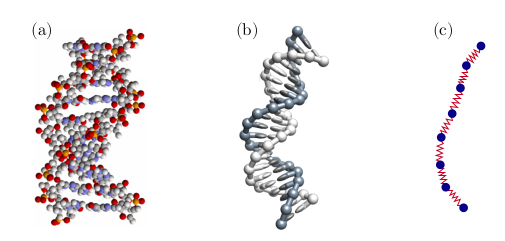
\includegraphics[width=0.8\linewidth]{Figures/CoarseGrained.png}
    \caption{zelf nog namaken met blender!!!}%
    \label{fig:Figures/CoarseGrained}
\end{figure}
 \cleardoublepage
\chapter{nano pore}
asldfkasdflj
 \cleardoublepage
\chapter{Methods}

\section{Figures}
An example is Figure~\ref{Landslide}
\begin{figure}[h] % [h] bepaalt de plaats waar de figuur komt in de tekst
    \centering % figuur komt in het midden terecht
    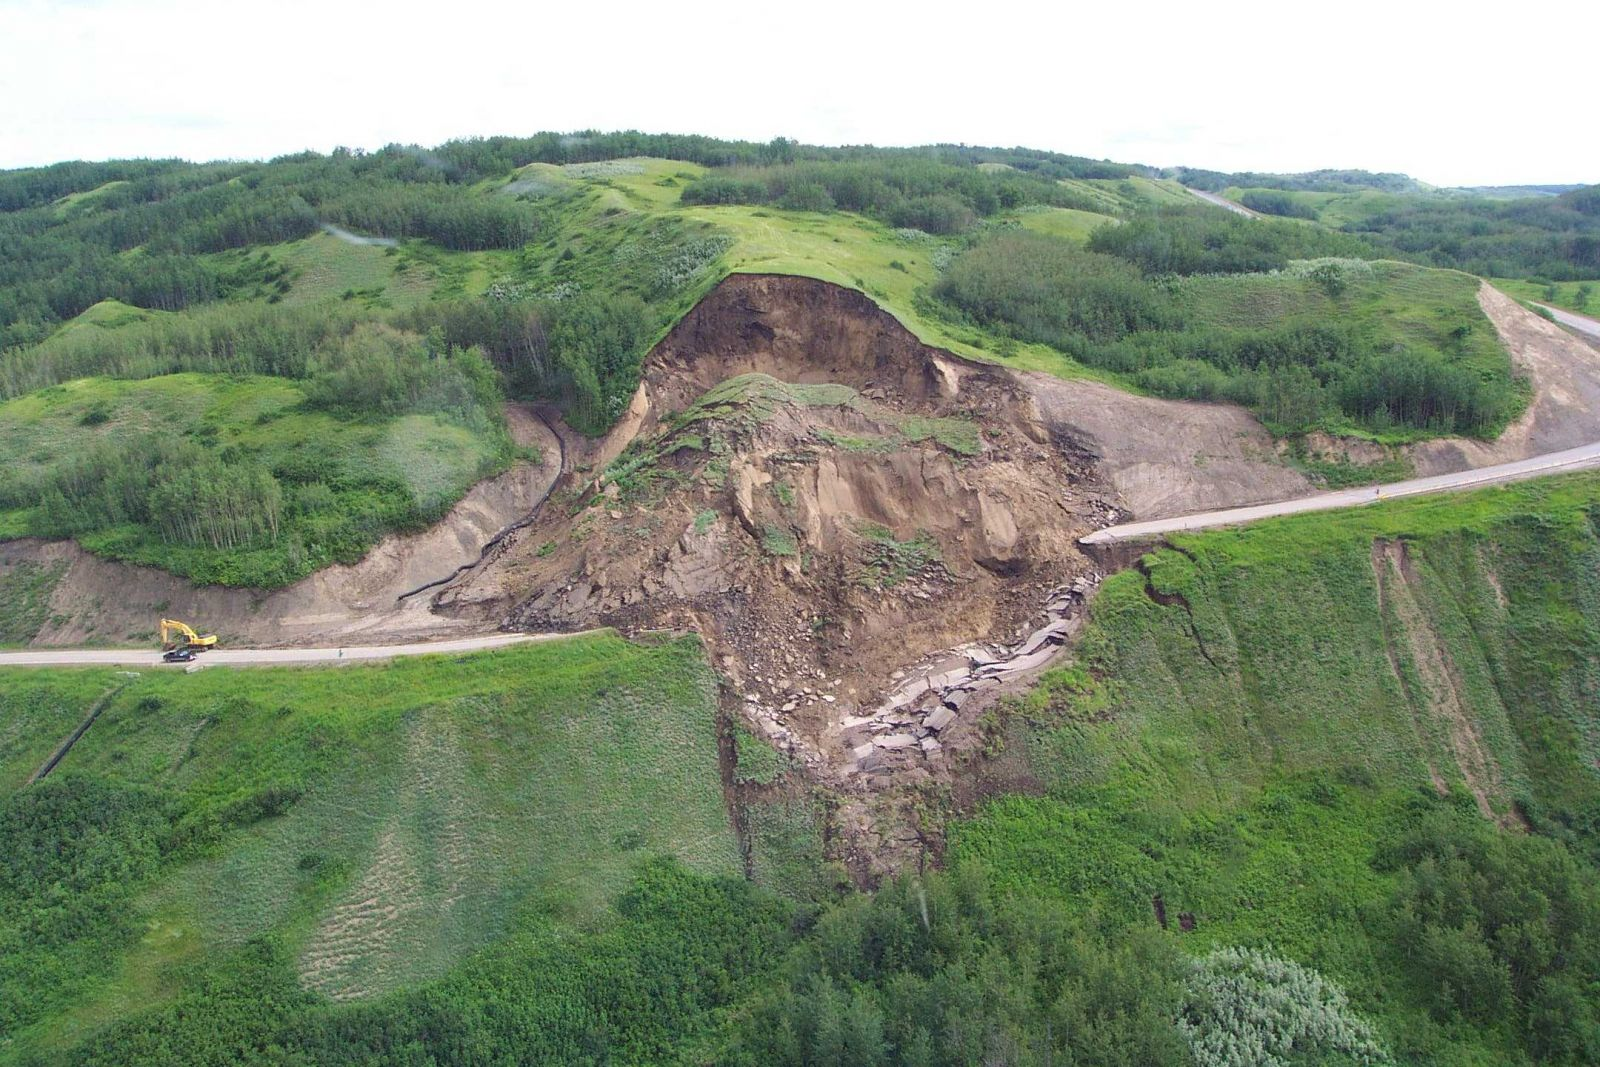
\includegraphics[width=0.8\textwidth]{Figures/landslide3.jpg}
    \caption{A landslide.}
    \label{Landslide}
\end{figure}

\newpage

\section{Tables}
An example is Table~\ref{Tabel1}
\begin{table}[h]
    \centering
    \begin{tabular}{|c|c|}
        \hline
       \bf Model  & \bf Accuracy  \\ \hline
        regression & 90\%                \\ \hline
        random forests & 95\%           \\ \hline
    \end{tabular}
    \caption{A random table.}
    \label{Tabel1}
\end{table}

\newpage

\section{Equations}
Equations can be inserted in the text itself, working in the \textit{mathmode}(put text between \$-signs, for example $Y_i=\frac{1}{x}$). Or put them in the text as a numbered floating element (e.g.\ Equation~\eqref{Eq1}).
\begin{equation}\label{Eq1}
    y=\frac{1}{x}
\end{equation}

\begin{equation}
    y=\int_{a}^{b} x^2 dx
\end{equation}

\begin{equation}
    y=\sum_{i=1}^{n} x_i^2
\end{equation}

You can align the equations:

\begin{align}
    y &=\frac{1}{x} \\
    y &=\int_{a}^{b} x^2 dx \\
    y &=\sum_{i=1}^{n} x_i^2
\end{align} \cleardoublepage
\chapter{Rotaxane}
\section{Mixed Rotaxane}

\subsection{Diffusion approximation}

Studying the dynamics of the mixed rotaxane highlighted the importance of entropic
interactions between the nano pore and the DNA strand. Here we observed that a fully
double stranded DNA polymer represented a special case. The uniformity of the
$\mathcal{X}$ histogram corresponding to this 0 nt mixed rotaxane suggests a free
diffusive motion of the rotaxane in a bounded one-dimensional domain. This isotropic
behaviour was previously also observed in the bead-spring simulations by Bayoumi et
al. \cite{EntropicPiston}\\

\begin{align*}
  \langle \Delta x^2 \rangle \simeq 2n Dt.
\end{align*}


\begin{align*}
  \frac{\partial \psi}{\partial t} =  D \frac{\partial^2 \psi}{\partial x^2}, P(x,t) =
f(x)g(t)
\end{align*}

\begin{align*}
\end{align*}

Reflecting boundary conditions $j = - D \frac{\partial \psi}{\partial x} = 0$. Current
vanishes at the boundaries

\begin{align*}
t:\quad \dot{g} = - \alpha g(t) \Rightarrow g(t) = e^{-\alpha t}
\end{align*}

\begin{align*}
  x:\quad D \ddot{f} = - \alpha f(x) \Rightarrow f(x) &= A \sin(K x) + B \cos(Kx)\\
  &= B \cos(\frac{\pi n x}{L})
\end{align*}
\begin{align*}
  \frac{\alpha}{D} = \frac{\pi^2 n^2}{L^2}
\end{align*}

The general solution is given by the linear combination,

\begin{align*}
  \psi(x,t) &= \sum_{n=0}^{+\infty} C_n \cos\Big(\frac{\pi n x}{L}\Big) e^{- \frac{D\pi^2
  n^2}{L^2}t}\\
            &=\frac{1}{L} \Bigg\{ 1 + \sum_{n=1}^{+\infty} \cos\Big(\frac{\pi n
  x_0}{L}\Big) \cos\Big(\frac{\pi n x}{L}\Big) e^{- \frac{D\pi^2  n^2}{L^2}t}\Bigg\}
\end{align*}
\begin{align*}
  \langle \Delta x^2 \rangle &= \langle(x-x_0)^2\rangle\\&= \frac{L^2}{6}(1 -
  \frac{96}{\pi^4}
  \sum_{n=0}^{+\infty} \frac{1}{(2k+1)^4} e^{- \frac{D(2k+1)^2 \pi^2}{L^2}t})\\
\end{align*}
As expected, the mean squared distances saturates to $\langle \Delta x^2 \rangle = L^2/6$
in the long-time limit $t \gg L^2 / D.$
 \cleardoublepage
\chapter{hybrydisation}
asldfkasdflj
 \cleardoublepage
\chapter{Conclusions and Perspectives}
\subsection{asdf}
 \cleardoublepage

% APPENDIX
\begin{appendices}
\addtocontents{toc}{\protect\setcounter{tocdepth}{1}}
\chapter{One Dimensional Confined Diffusion}

This appendix provides a detailed description of the motion of a Brownian particle
confined to a one dimensional domain. Due to the stochastic nature of this motion, we
will discuss the evolution of the probability density function $\phi(x,t)$, which
represents the probability of finding the particle on the position $x$ at time t.
Once the evolution of this probability function is known, the statistical properties can
be evaluated. Here, we will discuss the Mean Square Displacement (MSD), as it is used to
analyse the motion of the $0nt$ mixed rotaxane.\\
A central result in statistical mechanics is that the evolution of
$\phi$ is  described by the diffusion equation, given by
\begin{equation}
  \frac{\partial \psi}{\partial t} =  D \frac{\partial^2 \psi}{\partial x^2}, \quad
  \label{eq:diff}
\end{equation}
where D is the diffusion coefficient of our particle.
The confinement is imposed through reflecting boundary conditions at $x=0$ and $x=L$,
which is equivalent to imposing a
vanishing particle current at the boundaries of our domain, $j = - D \frac{\partial
\psi}{\partial x} = 0$. Solving equation \ref{eq:diff} can be done using the
method of
separation of variables, where we assume that the solution can be expressed as $
\psi(x,t) = f(x)g(t)$. Upon this substitution Eq. \ref{eq:diff} becomes,
\begin{equation}
  \frac{\dot{g}}{g} = \frac{\ddot{f}}{f} = - \alpha,
\end{equation}
where the two expressions are implied to be constant since the variables are independent.
The partial differential equation is now treated as two seperate ordinary differential
equations, for which we find,

\begin{align}
t:\quad \dot{g} = - \alpha g(t) \Rightarrow g(t) = e^{-\alpha t},
\end{align}

\begin{align}
  x:\quad D \ddot{f} = - \alpha f(x) \Rightarrow f(x) &= A \sin(K x) + B \cos(Kx)\\
  &= B \cos(\frac{\pi n x}{L}).
\end{align}
In the latter expression the boundary conditions impose that $A=0$ and constrain the
parameters by the relation,
\begin{align}
  \frac{\alpha}{D} = \frac{\pi^2 n^2}{L^2}.
\end{align}
By substituting the found results into the assumed form of the solution, we find the
general solution to the confined diffusion equation as the linear combination,
\begin{align}
  \psi(x,t) &= \sum_{n=0}^{+\infty} C_n \cos\Big(\frac{\pi n x}{L}\Big) e^{- \frac{D\pi^2
  n^2}{L^2}t}.
\end{align}
At time $t=0$ the particle is assumed to be found at $x_0$ resulting in the initial
condition,
\begin{align}
  \psi(x, 0) = \delta(x-x_0) = \sum_{n=0}^{+ \infty} C_n \cos(\frac{\pi n x}{L}).
\end{align}
Imposing this initial condition on the found general solution of the confined diffusion
equation gives,
\begin{align}
  \psi(x, t)=\frac{1}{L} \Bigg[ 1 + \sum_{n=1}^{+\infty} \cos\Big(\frac{\pi n
  x_0}{L}\Big) \cos\Big(\frac{\pi n x}{L}\Big) e^{- \frac{D\pi^2  n^2}{L^2}t}\Bigg].
\end{align}
This expression describes the behaviour of a Brownian particle in a one dimensional
confined domain. Using the found expression the MSD is calculated to be,
\begin{align}
  \langle \Delta x^2 \rangle &= \langle(x-x_0)^2\rangle\\&= \frac{L^2}{6}\Bigg[1 -
  \frac{96}{\pi^4}
  \sum_{k=0}^{+\infty} \frac{1}{(2k+1)^4} e^{- \frac{D(2k+1)^2 \pi^2}{L^2}t}\Bigg].
\end{align}
As expected, the mean square distances saturates to $\langle \Delta x^2 \rangle = L^2/6$
in the long-time limit $t \gg L^2 / D.$ To explore the other limiting case $t \ll L^2/D
$, we perform a Taylor expansion of the exponential and find,
\begin{align}
  \langle \Delta x^2 \rangle &= \frac{L^2}{6} - \frac{16 L^2}{\pi^4} \sum_{k=0}^{\infty}
  \frac{1}{(2k+1)^4} + \frac{16 D t}{\pi^2} \sum_{k=0}^{\infty} \frac{1}{(2k+1)^2} +
  \mathcal{O}\bigg(\frac{D^2 t^2}{L^4}\bigg).
\end{align}
Using the two convergent series,
\begin{equation}
  \sum_{k=0}^{\infty} \frac{1}{(2k+1)^2} = \frac{\pi^2}{8} \qquad \text{and} \qquad
  \sum_{k=0}^{\infty} \frac{1}{(2k+1)^4} = \frac{\pi^4}{96}
\end{equation}
the free diffusion is recovered at short time scales,\cite{BICKEL200724}
\begin{equation}
  \langle \Delta x^2 \rangle = 2Dt \qquad \text{for }\,\, t \ll L^2/D.
\end{equation}

\end{appendices}

% BIBLIOGRAPHY
%\addcontentsline{toc}{chapter}{Bibliography}
\bibliographystyle{apalike}
\begin{multicols}{2}
\begin{smallfont}
\bibliography{Bibliography/thesis.bib}
\end{smallfont}
\end{multicols}
\cleardoublepage

\chapter*{Acknowledgements}
\addcontentsline{toc}{chapter}{Acknowledgements}
...
 \cleardoublepage


% Back side of book
\cleartoleftpage{} % Make sure the back page is at an even page number


% ----------------------- Achterblad ------------------------------
% Vergeet niet de tekst aan te passen:
% - Afdeling
% - Adres van de afdeling
% - Telefoon en faxnummer
% -----------------------------------------------------------------
\thispagestyle{empty}
\sffamily
%
\begin{textblock}{191}(102,-22)
{\color{blueline}\rule{160pt}{5.5pt}}
\end{textblock}
%
\begin{textblock}{191}(157,-22)
{\color{blueline}\rule{5.5pt}{59pt}}
\end{textblock}
%
\begin{textblock}{183}(-35,-22)
\textblockcolour{}
\flushright
\fontsize{7}{7.5}\selectfont
\textbf{DEPARTEMENT NATUURKUNDE EN STERRENKUNDE}\\
Celestijnenlaan 200d bus 2412\\
3000 LEUVEN, BELGI\"{E}\\
tel. + 32 16 32 71 24\\
fys.kuleuven.be\\
\end{textblock}
%
\begin{textblock}{191}(145,-16)
\textblockcolour{}
\includegraphics*[height=16.5truemm]{Figures/sedes}
\end{textblock}
%
\begin{textblock}{191}(-31,224)
{\color{bluetitle}\rule{544pt}{55pt}}
\end{textblock}


\end{document}
